\documentclass[11pt,aspectratio=169]{beamer}
\usepackage[T5]{fontenc}
\usepackage[utf8]{inputenc}
\usepackage[vietnamese]{babel}
\usepackage{amsmath,amssymb,bm,mathtools}
\usetheme{CambridgeUS}
\usecolortheme{dolphin}
\usefonttheme{professionalfonts}
\setbeamertemplate{navigation symbols}{}
\setbeamerfont{section in toc}{series=\bfseries}
\setbeamerfont{subsection in toc}{series=\bfseries}
\usepackage{booktabs}
\usepackage{multirow}
\usepackage{tabularx}
\usepackage{array}
\usepackage{tikz}
\usepackage{graphicx}
\usetikzlibrary{arrows.meta,positioning,shapes.geometric,calc,fit,backgrounds}

\AtBeginSection[]
{
    \ifnum\value{section}>0\relax
        \begin{frame}{Mục lục phần}
            \tableofcontents[
            currentsection,
            sectionstyle=show/shaded,
            subsectionstyle=show/shaded/hide
        ]
        \end{frame}
    \fi
}

\AtBeginSubsection[]
{
    \ifnum\value{subsection}>0\relax
        \begin{frame}{Mục lục phần}
            \tableofcontents[
            currentsection,
            currentsubsection,
            sectionstyle=show/shaded,
            subsectionstyle=show/shaded/hide
        ]
        \end{frame}
    \fi
}

\setbeamertemplate{footline}[frame number]

\title{DoRA and LoRA \\
Implement from Beginning}
\author{3ChuBeDan}
\institute{Vietnam National University - University of Engineering and Technology\\Institute for Artificial Intelligence}
\date{\today}
\begin{document}

\begin{frame}
    \titlepage
\end{frame}

\begin{frame}{Dàn ý trình bày}
    \tableofcontents[sectionstyle=show,subsectionstyle=show/show/hide]
\end{frame}



\begin{frame}{Ba câu hỏi nghiên cứu}
\footnotesize
\begin{columns}[T]
\begin{column}{0.52\textwidth}
\textbf{Góc nhìn báo cáo}
\begin{itemize}
  \item Xây dựng PEFT from scratch thay vì chỉ dùng thư viện có sẵn.
  \item Kiểm nghiệm trên UIT-ViON với PhoBERT cho phân loại 13 chủ đề tin tức tiếng Việt.
  \item So sánh chi phí tài nguyên và chất lượng phân loại giữa FT, LoRA và DoRA.
\end{itemize}

\vspace{0.12cm}
\textbf{Ba câu hỏi chính}
\begin{enumerate}
  \item LoRA/DoRA có thể được cài đặt trực tiếp bằng PyTorch như thế nào?
  \item PEFT from scratch được tích hợp vào PhoBERT cho UIT-ViON ra sao?
  \item Trade-off giữa accuracy và chi phí tài nguyên là gì?
\end{enumerate}
\end{column}

\begin{column}{0.44\textwidth}
\centering
\begin{tikzpicture}[scale=0.72, every node/.style={transform shape}]
  \tikzstyle{block} = [rectangle, rounded corners, draw=blue!60, fill=blue!5, very thick,
                      minimum width=2.35cm, minimum height=0.65cm, align=center, font=\scriptsize\bfseries]
  \tikzstyle{arrow} = [->, thick, draw=gray!60]
  \node[block] (text) {Văn bản UIT-ViON};
  \node[block, below=0.32cm of text] (phobert) {PhoBERT};
  \node[block, below=0.32cm of phobert] (peft) {LoRA / DoRA};
  \node[block, below=0.32cm of peft] (cls) {Classifier};
  \node[block, below=0.32cm of cls] (out) {13 chủ đề};
  \draw[arrow] (text) -- (phobert);
  \draw[arrow] (phobert) -- (peft);
  \draw[arrow] (peft) -- (cls);
  \draw[arrow] (cls) -- (out);
  \node[font=\scriptsize, text=blue!70!black, right=0.15cm of peft] {$\leftarrow$ hiệu quả tham số};
\end{tikzpicture}
\end{column}
\end{columns}
\end{frame}





\section{LoRA - Parameter-Efficient Fine-Tuning - Tinh chỉnh tham số hiệu quả}
\subsection{LoRA - Parameter-Efficient Fine-Tuning (PEFT)}
\begin{frame}[t]{LoRA - Parameter-Efficient Fine-Tuning - Tinh chỉnh tham số hiệu quả (PEFT)}
\scriptsize
\begin{itemize}
\item Dựa trên giả thuyết cho rằng các thay đổi được tạo ra trong quá trình tinh chỉnh có 'hạng nội tại' (intrinsic rank) thấp, LoRA (Hu et al.,
2022) đề xuất sử dụng tích của hai ma trận hạng thấp để cập nhật trọng số tiền huấn luyện. LoRA giải quyết chi phí của FFT bằng cách đóng băng ma trận tiền huấn luyện $W_0\in\mathbb{R}^{d\times k}$ và chỉ học cách hiệu chỉnh phần thích nghi $\Delta W$.
\item Trọng số sau thích nghi được viết:
$$
W' = W_0 + \Delta W = W_0 + BA.
$$
\item Trong đó:
$$
B\in\mathbb{R}^{d\times r}, \quad A\in\mathbb{R}^{r\times k}, \quad r\ll \min(d,k).
$$
\item Thay vì học $d\times k$ tham số, LoRA chỉ học:
$$
\#\text{params}_{\text{LoRA}}=r\times (d+k)\ll d\times k.
$$
\item Phương pháp này hiệu quả nhất khi cập nhật theo tác vụ nằm gần một không gian con thấp chiều của không gian tham số đầy đủ.
\item Vì ma trận $W_0$ được giữ cố định, tri thức tiền huấn luyện được bảo toàn trực tiếp hơn và kích thước checkpoint nhỏ hơn nhiều.
\end{itemize}
\end{frame}

\subsection{Nút thắt hình học của LoRA}
\begin{frame}[t]{Nút thắt hình học của LoRA}
\footnotesize

\begin{itemize}
    \item Mặc dù LoRA hiệu quả về mặt tham số, nhưng độ chính xác của nó không tương đương với tinh chỉnh toàn phần (full fine-tuning).
    \item Thành phần hiệu chỉnh cộng bị giới hạn trong không gian con hạng thấp:
    $$
        W' = W_0 + BA, \quad \Delta W \in \mathcal{S}_r, \quad \text{dim}(\mathcal{S}_r) \ll d \times k
    $$
    \item Để dễ hình dung, ta có thể coi bộ tối ưu (optimizer) chỉ khám phá một \textbf{đa tạp con thấp chiều} (low-dimensional submanifold) bên trong không gian tham số đầy đủ:
    $$\Delta W = \{BA | B \in \mathbb{R}^{d \times r}, A \in \mathbb{R}^{r \times k}\}$$
    \item Trong hình học của LoRA, các thay đổi về độ lớn và hướng của véc-tơ trọng số bị 'khóa' chặt vào nhau bên trong một đa tạp con thấp chiều. Do đa tạp này có số chiều cực thấp, bộ tối ưu không thể di chuyển độc lập theo một hướng để thay đổi độ lớn mà không làm lệch hướng khiến thay đổi cấu trúc đặc trưng. Điều này tạo ra một sự ràng buộc hình học khắt khe, khiến mô hình khó lòng đạt được cấu hình trọng số tối ưu như trong không gian Euclid tự do của việc tinh chỉnh toàn phần (FFT).
    \item Sự sai lệch này trở nên trầm trọng khi hạng $r$ nhỏ và tác vụ yêu cầu những thay đổi phức tạp trong hình học biểu diễn.
\end{itemize}
\end{frame}

\section{DoRA: : Weight-Decomposed Low-Rank Adaptation}
\subsection{Nền tảng toán học - Weight Normalization}
\begin{frame}[t]{Nền tảng toán học - Weight Normalization}
\footnotesize
\begin{itemize}
\item Lấy ý tưởng từ Weight Normalization (Salimans
\& Kingma, 2016), DoRA đi theo ý tưởng tách biệt độ lớn của vector trọng số khỏi hướng của nó.
\item Trong Weight Normalization, mỗi cột $j$ của ma trận trọng số được phân rã thành:
$$
\bm{w}_j = m_j \frac{\bm{v}_j}{\|\bm{v}_j\|_2}.
$$
\item Trong đó: $m_j$ là đại lượng vô hướng điều khiển độ lớn, và $\bm{v}_j/\|\bm{v}_j\|_2$ là vector đơn vị dùng để xác định hướng. ($\||\cdot||_2$ là chuẩn L$^2$ - Euclidean norm).
\item Cách tiếp cận này thay đổi \textbf{cách cập nhật hình học của quá trình tối ưu}: độ lớn thay đổi dọc theo bán kính, trong khi hướng di chuyển trên mặt cầu đơn vị.
\item Sự phân rã này giúp tách rời hai vai trò khác nhau của trọng số vốn bị \textbf{ràng buộc chặt chẽ} trong cách tham số hóa của LoRA, cho phép mô hình học được các quỹ đạo tối ưu hóa linh hoạt hơn.
\item \textbf{Trực giác:} Việc cập nhật độ lớn và hướng bằng hai cơ chế riêng biệt giúp mô hình thích nghi hiệu quả hơn với dữ liệu mới.
\end{itemize}
\end{frame}




\subsection{Kiến trúc toán học của DoRA}
\begin{frame}[t]{Kiến trúc toán học của DoRA}
\scriptsize
\begin{itemize}
    \item Bảo toàn tri thức tiền huấn luyện: DoRA đảm bảo điểm khởi đầu nhất quán với mô hình gốc bằng cách thiết lập:$$V = W_0, \quad m = \|W_0\|_c,$$
trong đó, $\|\cdot\|_c$ là chuẩn Euclid ($L^2$ norm) tính toán độc lập trên từng cột của ma trận trọng số (column-wise norm).
    \item Tái tham số hóa thành phần hướng: Nhánh thích nghi theo hướng (directional component) kế thừa cấu trúc của LoRA để cập nhật ma trận $V$ một cách hiệu quả về tham số. DoRA, khi đó, được thiết lập theo công thức của phân rã trọng số, $W = m \frac{V}{\|V\|_c} = \left\|W\right\|_c \frac{W}{\left\|W\right\|_c}$
như sau:
$$W' = m \frac{V + \Delta V}{\|V + \Delta V\|_c} = m \frac{W_0 + BA}{\|W_0 + BA\|_c}.$$
Trong đó $m, B, A$ là các tham số có thể huấn luyện (trainable parameters).

\end{itemize}
\end{frame}

\begin{frame}[t]{Đặc điểm hình học của DoRA}
$$W' = m \frac{V + \Delta V}{\|V + \Delta V\|_c} = m \frac{W_0 + BA}{\|W_0 + BA\|_c}$$
\begin{itemize}
\item Loại bỏ sự ràng buộc giữa hướng và độ lớn: Trong cấu trúc này, hạng tử hạng thấp ($BA$) tập trung chuyên biệt vào việc tinh chỉnh \textbf{hướng} (direction), trong khi vector $m$ đảm nhận vai trò điều chỉnh \textbf{độ lớn} (magnitude) một cách độc lập.

\item Tính ổn định tại thời điểm khởi tạo: Nhờ thiết kế chuẩn hóa, tại bước $t=0$, mô hình DoRA khôi phục chính xác trạng thái của mô hình $W_0$.

\item Mở rộng năng lực biểu đạt: Thiết kế này không chỉ duy trì tính hiệu quả của PEFT (Parameter-Efficient Fine-Tuning) mà còn giải phóng mô hình khỏi các ràng buộc hình học của LoRA chuẩn, cho phép quỹ đạo tối ưu hóa tiến gần hơn với tinh chỉnh toàn phần (Full Fine-tuning).
\end{itemize}

\end{frame}


\subsection{Phân tích Gradient của DoRA}
\begin{frame}[t]{Gradient của DoRA}
\footnotesize
Xét quá trình lan truyền ngược qua phân rã trọng số $W = m \frac{V}{\|V\|_c}$. Theo quy tắc dây chuyền, gradient đối với thành phần hướng $V'=V+\Delta V$ và độ lớn $m$ là:
    \begin{align}
        &\nabla_{V'} \mathcal{L} = \frac{m}{\|V\|_c} \left( I - \frac{V' V'^T}{\|V'\|_c^2} \right) \nabla_{W'} \mathcal{L} \label{eq:gradient-wrt-direction} \\
        &\nabla_{m} \mathcal{L} = \frac{ \nabla_{W'} \mathcal{L} \cdot V'}{\|V'\|_c} \label{eq:gradient-wrt-magnitude}
    \end{align}
\end{frame}



\subsection{Đột phá hình học - Phép chiếu trực giao}
\begin{frame}[t]{Đột phá hình học - Phép chiếu trực giao}
\scriptsize
\begin{itemize}
    \item Từ phương trình (\ref{eq:gradient-wrt-direction}), ta có thể định nghĩa toán tử chiếu trực giao $P$:
    $$P = I - \frac{V'V'^T}{\|V'\|_c^{2}}$$
    \item Toán tử này loại bỏ hoàn toàn thành phần xuyên tâm vì:
    $$PV' = V' - \frac{V'(V'^T V')}{\|V'\|_c^{2}} = V' - V' = 0$$
    \item Suy ra, gradient đối với thành phần hướng $\nabla_{V'}\mathcal{L} \propto P \nabla_{W'}\mathcal{L}$ luôn nằm trong không gian tiếp tuyến trực giao với $V'$:
    $$V'^T \nabla_{V'}\mathcal{L}=0$$
    \item \textbf{Ý nghĩa hình học:} Nhờ vào tính trực giao, DoRA thiết lập một cơ chế tách biệt hoàn toàn: việc xoay hướng trọng số không còn làm biến động độ lớn, và ngược lại, việc điều chỉnh độ lớn không làm sai lệch hướng. Sự độc lập này cho phép mô hình tối ưu hóa từng thành phần một cách tinh tế, loại bỏ sự ràng buộc gây nhiễu vốn là điểm yếu cố hữu của LoRA chuẩn.
\end{itemize}
\end{frame}


\subsection{Phân tích Động học: Tương quan nghịch giữa Hướng và Độ lớn}
% --- SLIDE 1: THIẾT LẬP CÔNG THỨC ---

\begin{frame}[t]{Phân tích Động học (I)}
    \scriptsize
    \textit{Ở đây, ta sử dụng các kí hiệu chữ cái viết thường cho vector thay vì các kí hiệu ma trận như các slide trước. Việc chuyển sang ký hiệu vector chữ thường nhằm phân tích hành vi hình học độc lập của từng cột trọng số (tương ứng với mỗi neuron), giúp đơn giản hóa việc chứng minh các thuộc tính về hướng và độ lớn.}

    Xét cập nhật tham số cho các trọng số: $w'' = w' + \Delta w$ với $\Delta w \propto \nabla_{w'} \mathcal{L}$.

    \textbf{Giả thuyết so sánh:} Xét hai kịch bản cập nhật $S_1$ và $S_2$, với $\Delta D_{S_1} < \Delta D_{S_2}$ (kịch bản $S_1$ có bước nhảy về hướng nhỏ hơn).
    
    Giả sử $\|\Delta w_{S_1}\| =  \|\Delta w_{S_2}\|$, và tại thời điểm ban đầu, ta có $\Delta v = 0$ và $v' = v$.
    
    Từ điều kiện $\Delta D_{S_1} < \Delta D_{S_2}$, ta có $|\cos(\Delta w_{S_1}, w')| > |\cos(\Delta w_{S_2}, w')|$.

    Vì $\Delta w \propto \nabla_{w'} \mathcal{L}$, ta có $\left|\cos\left(\nabla_{w'}^{S_1} \mathcal{L}, w'\right)\right| > \left|\cos\left(\nabla_{w'}^{S_2} \mathcal{L}, w'\right)\right|$.

    Với việc khởi tạo $v = v_0$ và $w'=w_0$ tại thời điểm ban đầu, ta có thể thay thế $w'$ bằng $v$ trong biểu thức cosine, dẫn đến $|\cos(\nabla_{w'}\mathcal{L}, w')| = |\cos(\nabla_{w'}\mathcal{L}, v')| = |\cos(\nabla_{w'}\mathcal{L}, v)|$.

    Với $\Delta v = 0$, ta có $$|\cos(\nabla_{w'}\mathcal{L}, w')| = |\cos(\nabla_{w'}\mathcal{L}, v')| = |\cos(\nabla_{w'}\mathcal{L}, v)| = \frac{\nabla_{w'}\mathcal{L}\cdot v}{\|\nabla_{w'}\mathcal{L}\| \|v\|}.$$


\end{frame}

% --- SLIDE 2: CHỨNG MINH HỆ QUẢ ---
\begin{frame}[t]{Phân tích Động học (II)}
    \scriptsize
        Gọi $m_{*}$ là tham số độ lớn của vector $w'$, khi đó phương trình (\ref{eq:gradient-wrt-magnitude}) có thể viết lại thành:
    $$\nabla_{m_{*}} \mathcal{L} = \frac{\nabla_{w'} \mathcal{L} \cdot v'}{\|v'\|_c} = \left\|\nabla_{w'} \mathcal{L}\right\| \cdot \cos(\nabla_{w'} \mathcal{L}, v)$$
    
    Bởi $\|\Delta w_{S_1}\| =  \|\Delta w_{S_2}\|$, ta có $\left\|\nabla_{w'}^{S_1} \mathcal{L}\right\| = \left\|\nabla_{w'}^{S_2} \mathcal{L}\right\|$. Do đó, với $|\cos(\nabla_{w'}^{S_1} \mathcal{L}, v)| > |\cos(\nabla_{w'}^{S_2} \mathcal{L}, v)|$, ta có 
    
    $$\left|\nabla_{m_{*}}^{S_1} \mathcal{L}\right| > \left|\nabla_{m_{*}}^{S_2} \mathcal{L}\right|.$$
    \begin{itemize}
    \item \textbf{Hệ quả trực tiếp:}
    $$
        \Delta D_{S_1} < \Delta D_{S_2} \implies \left|\nabla_{m_{*}}^{S_1} \mathcal{L}\right| > \left|\nabla_{m_{*}}^{S_2} \mathcal{L}\right|
    $$
    
    \item \textbf{Phân tích kết quả:}
    \begin{itemize}
        \item $S_1$: Thay đổi hướng \textbf{ít} $\implies$ Cập nhật độ lớn \textbf{nhiều}.
        \item $S_2$: Thay đổi hướng \textbf{nhiều} $\implies$ Cập nhật độ lớn \textbf{ít}.
    \end{itemize}
\end{itemize}

\begin{block}{Kết luận: Sự tự điều tiết của DoRA}
DoRA thiết lập mối tương quan nghịch giữa hướng và độ lớn. Khi mô hình cần thay đổi đặc trưng mạnh mẽ (xoay hướng), nó sẽ tự động kìm hãm sự biến động về cường độ (độ lớn).
\end{block}
\end{frame}


\subsection{Tối ưu hóa bộ nhớ: Cơ chế Detached Gradient}
\begin{frame}[t]{Tối ưu hóa bộ nhớ: Cơ chế Detached Gradient}
\scriptsize

\begin{columns}[T] % T: căn chỉnh nội dung lên phía trên

    % --- CỘT TRÁI: VẤN ĐỀ VÀ GIẢI PHÁP ---
    \begin{column}{0.55\textwidth}
        \textbf{Vấn đề: Chi phí bộ nhớ (VRAM)}
        \begin{itemize}
            \item Gradient nhánh hướng (\ref{eq:gradient-wrt-direction}) khác biệt so với $W'$, buộc đồ thị tính toán lưu nhiều biến trung gian.
            \item Gây tăng mức tiêu thụ VRAM đáng kể trong Backpropagation.
        \end{itemize}
Nhóm nghiên cứu đã đề xuất giải pháp để khắc phục vấn đề này mà không làm mất đi tính hiệu quả của DoRA.

        \vspace{0.2cm}
        \textbf{Giải pháp: Detaching $\|V'\|_c$}
        \begin{itemize}
            \item Coi $\|V + \Delta V\|_c$ là \textbf{hằng số} khi tính đạo hàm.
            \item \textbf{Forward:} Cập nhật giá trị động.
            \item \textbf{Backward:} Ngắt khỏi đồ thị gradient (không truyền đạo hàm qua chuẩn $c$).
        \end{itemize}
    \end{column}

    % --- CỘT PHẢI: CÔNG THỨC VÀ KẾT QUẢ ---
    \begin{column}{0.4\textwidth}
        \textbf{Công thức rút gọn:}
        $$
            \nabla_{V'} \mathcal{L} = \frac{m}{C} \nabla_{W'} \mathcal{L}
        $$
        \begin{center}
            \textit{với $C = \|V'\|_c$ (detached)}
        \end{center}
        

    \end{column}

\end{columns}

\vspace{0.3cm}
\begin{block}{Kết luận}
Cơ chế này đưa chi phí bộ nhớ của DoRA nhỏ hơn nhưng vẫn giữ được ưu thế hội tụ của Full Fine-tuning.
\end{block}

\end{frame}

\begin{frame}[fragile]{Mã giả – DoRA Forward}
\footnotesize
\begin{columns}[T]

\begin{column}{0.48\textwidth}
\textbf{Thuật toán \texttt{merged\_weight}}
\begin{enumerate}
\item $\Delta \gets BA \times \frac{\alpha}{r}$
\item $V \gets W_0 + \Delta$
\item $\mathbf{n} \gets \|V\|_c$ \hfill (chuẩn cột)
\item \textbf{Nếu} detach: $\mathbf{n} \gets \mathbf{n}.\text{detach}()$
\item $\mathbf{n} \gets \max(\mathbf{n}, \varepsilon)$
\item \textbf{Trả về} $m \odot V \oslash \mathbf{n}$ \hfill (nhân/chia theo cột)
\end{enumerate}
\end{column}

\begin{column}{0.48\textwidth}
\textbf{Thuật toán \texttt{forward}}
\begin{enumerate}
\item \textbf{Nếu} merged:
   \begin{itemize}
   \item Trả về $\text{Linear}(x, W_0, b)$
   \end{itemize}
\item \textbf{Nếu} không bật adapter:
   \begin{itemize}
   \item Trả về $\text{Linear}(x, W_0, b)$
   \end{itemize}
\item $W' \gets \text{merged\_weight}()$
\item Trả về $\text{Linear}(x, W', b)$
\end{enumerate}
\end{column}

\end{columns}
\end{frame}




\begin{frame}[fragile]{Mã giả – apply\_peft \& Quản lý Adapter}
\footnotesize
\begin{columns}[T]

\begin{column}{0.48\textwidth}
\textbf{Hàm \texttt{apply\_peft}}
\begin{enumerate}
\item \textbf{Với mỗi} module\_name, module trong model:
   \begin{enumerate}
   \item \textbf{Nếu} tên khớp với target\_modules và module là Linear:
      \begin{itemize}
      \item Tạo LoRALinear hoặc DoRALinear
      \item Thay thế module cha
      \end{itemize}
   \end{enumerate}
\item \textbf{Trả về} danh sách tên module đã thay thế
\end{enumerate}
\end{column}

\begin{column}{0.48\textwidth}
\textbf{Lưu / Tải adapter}
\begin{enumerate}
\item \textbf{Lưu:}
   \begin{enumerate}
   \item Thu thập các tham số huấn luyện được (lora\_A, lora\_B, magnitude,…)
   \item Lưu vào file với tên module tương ứng
   \end{enumerate}
\item \textbf{Tải:}
   \begin{enumerate}
   \item Đọc file đã lưu
   \item Với mỗi module trong file:
      \begin{itemize}
      \item Sao chép tham số vào module tương ứng trong model hiện tại
      \end{itemize}
   \end{enumerate}
\end{enumerate}
\end{column}

\end{columns}
\end{frame}


\section{Kết quả thực nghiệm}

\begin{frame}{Thiết lập benchmark UIT-ViON}
\footnotesize
\begin{columns}[T]
\begin{column}{0.48\textwidth}
\textbf{Dữ liệu và mô hình}
\begin{itemize}
  \item Dataset: UIT-ViON subset, file \texttt{data/uit\_vion/subset.csv}.
  \item Bài toán: phân loại single-label với 13 chủ đề.
  \item Backbone: \texttt{vinai/phobert-base-v2}.
  \item Mỗi cấu hình chạy với ba seed: 97, 98, 99.
\end{itemize}
\end{column}

\begin{column}{0.48\textwidth}
\textbf{Cấu hình so sánh}
\begin{itemize}
  \item FT: fine-tune toàn bộ PhoBERT.
  \item LoRA/DoRA: rank 8 và 16, $\alpha = 2r$.
  \item Target modules: \texttt{query}, \texttt{value}.
  \item Metric chính: accuracy; macro-F1/weighted-F1 dùng để audit.
\end{itemize}
\end{column}
\end{columns}

\vspace{0.25cm}
\centering
\scriptsize
\begin{tabular}{llll}
\toprule
Nhóm & Method & Rank & Nguồn kết quả \\
\midrule
Baseline & FT & full & \texttt{benchmark\_results\_2.csv} \\
PEFT from scratch & LoRA, DoRA & 8, 16 & \texttt{benchmark\_results\_2.csv} \\
PEFT official & FT, LoRA, DoRA & full, 8, 16 & \texttt{offical\_benchmark\_result.csv} \\
\bottomrule
\end{tabular}
\end{frame}

\begin{frame}{Kết quả PEFT from scratch trên UIT-ViON}
\centering
\scriptsize
\begin{tabular}{lrrrrr}
\toprule
Method & Acc. & Train. \% & Time (s) & VRAM (MB) & Ckpt (MB) \\
\midrule
FT & 0.8109 & 100.00 & 513.0 & 2089 & 8253 \\
LoRA r8 & 0.7982 & 0.66 & 260.2 & 773 & 3.43 \\
LoRA r16 & 0.7987 & 0.88 & 302.0 & 777 & 4.56 \\
DoRA r8 & 0.8031 & 0.75 & 276.9 & 871 & 3.51 \\
DoRA r16 & 0.8036 & 1.00 & 267.2 & 874 & 4.64 \\
\bottomrule
\end{tabular}

\vspace{0.25cm}
\begin{minipage}{0.86\textwidth}
\footnotesize
FT đạt accuracy trung bình cao nhất nhưng cần huấn luyện toàn bộ tham số và tạo checkpoint rất lớn.
LoRA/DoRA chỉ huấn luyện dưới 1\% tham số, giảm checkpoint xuống mức vài MB trong khi accuracy vẫn gần baseline.
\end{minipage}
\end{frame}

\begin{frame}{So sánh với PEFT official}
\centering
\scriptsize
\begin{tabular}{lrrrrr}
\toprule
Method & Custom acc. & Official acc. & $\Delta$ acc. (pp) & $\Delta$ time (s) & $\Delta$ VRAM (MB) \\
\midrule
FT & 0.8109 & 0.8109 & 0.000 & -27.7 & 0.5 \\
LoRA r8 & 0.7982 & 0.7971 & -0.115 & 10.8 & 530.5 \\
LoRA r16 & 0.7987 & 0.8028 & 0.410 & -62.7 & 2.4 \\
DoRA r8 & 0.8031 & 0.7973 & -0.577 & 58.1 & -44.0 \\
DoRA r16 & 0.8036 & 0.8009 & -0.269 & 86.7 & -43.7 \\
\bottomrule
\end{tabular}

\vspace{0.25cm}
\begin{minipage}{0.86\textwidth}
\footnotesize
Các delta được tính theo \textbf{official - custom} và ghép cặp theo method, rank, seed.
Khác biệt accuracy trung bình nằm dưới 1 điểm phần trăm, cho thấy bản cài đặt from scratch bám sát hành vi của PEFT official trong benchmark này.
\end{minipage}
\end{frame}

\begin{frame}{Biểu đồ so sánh tài nguyên}
\centering
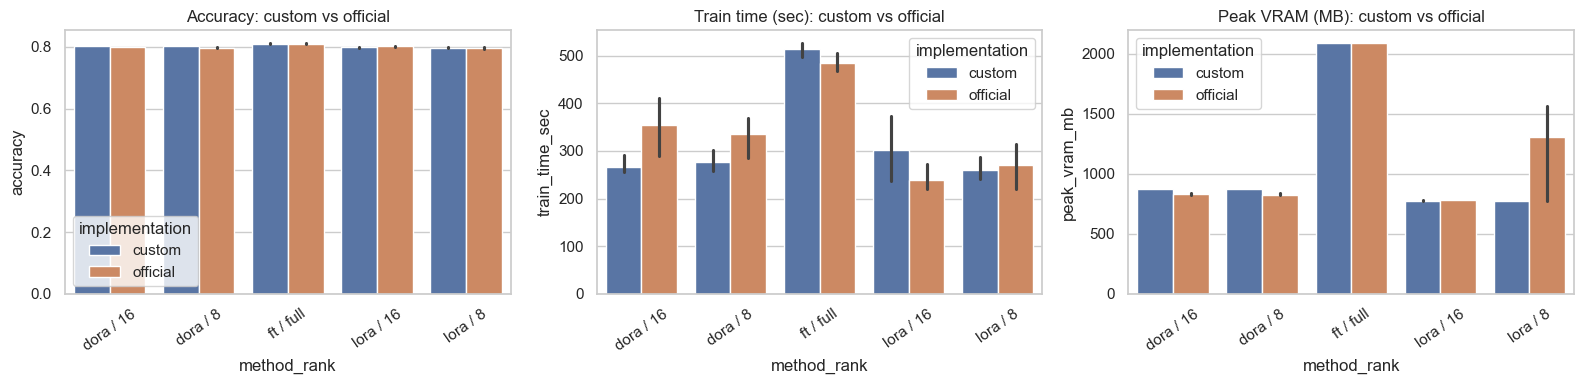
\includegraphics[width=0.95\textwidth,height=0.36\textheight,keepaspectratio]{../results/performance.png}

\vspace{0.12cm}
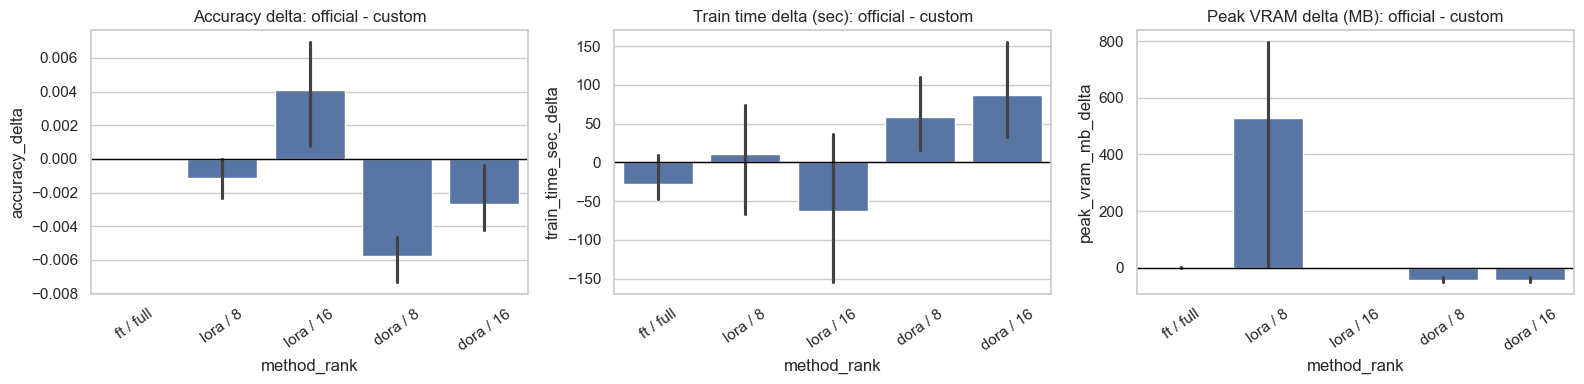
\includegraphics[width=0.95\textwidth,height=0.36\textheight,keepaspectratio]{../results/performance2.png}

\vspace{0.08cm}
\scriptsize
Các biểu đồ tập trung vào accuracy, thời gian huấn luyện, VRAM đỉnh và kích thước checkpoint; macro-F1 không dùng làm graph chính cho thiết lập single-label.
\end{frame}

\begin{frame}{Scatter paired accuracy}
\footnotesize
\begin{columns}[T]
\begin{column}{0.54\textwidth}
\centering
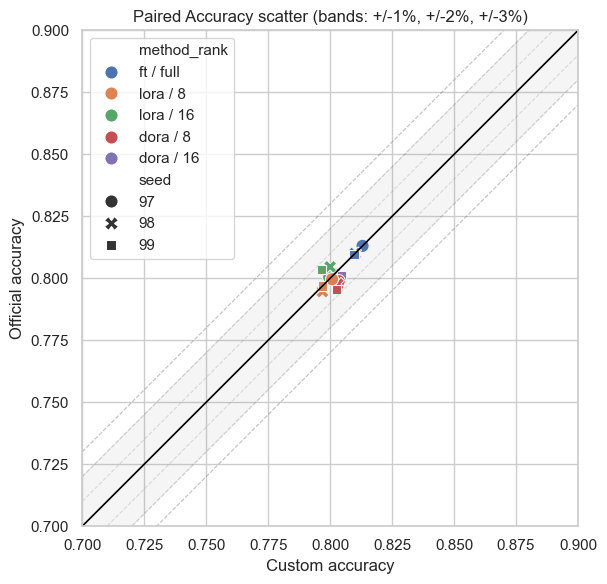
\includegraphics[width=\textwidth,height=0.74\textheight,keepaspectratio]{../results/scatterplot.png}
\end{column}

\begin{column}{0.42\textwidth}
\textbf{Cách đọc biểu đồ}
\begin{itemize}
  \item Mỗi điểm là một cặp chạy cùng method, rank và seed.
  \item Đường $x=y$ biểu thị official và custom có accuracy bằng nhau.
  \item Các dải tham chiếu $\pm$1\%, $\pm$2\%, $\pm$3\% giúp tránh phóng đại chênh lệch nhỏ.
  \item Các điểm nằm gần $x=y$, khác biệt rõ chỉ khi vượt khoảng 2--3\%.
\end{itemize}
\end{column}
\end{columns}
\end{frame}


\section{Tài liệu tham khảo}
\begin{frame}[allowframebreaks]{Tài liệu tham khảo}
\scriptsize
\begin{thebibliography}{3}

\bibitem{dora2024}
Shih-Yang Liu, et al.
\newblock \textbf{DoRA: Weight-Decomposed Low-Rank Adaptation}.
\newblock \textit{arXiv preprint arXiv:2402.09353}, 2024.

\bibitem{lora2021}
Edward J. Hu, et al.
\newblock \textbf{LoRA: Low-Rank Adaptation of Large Language Models}.
\newblock \textit{ICLR}, 2022.

\bibitem{weightnorm2016}
Tim Salimans and Diederik P. Kingma.
\newblock \textbf{Weight Normalization: A Simple Reparameterization to Accelerate Training of Deep Neural Networks}.
\newblock \textit{Advances in Neural Information Processing Systems}, 2016.

\end{thebibliography}
\end{frame}

{
\begin{frame}[plain]
    \begin{center}
        \vspace{2.5cm}
        \Huge \textbf{TRÂN TRỌNG CẢM ƠN!}
        
        \vspace{1cm}
        \normalsize 
        \textbf{PHẦN THẢO LUẬN (Q\&A)}

    \end{center}
\end{frame}
}



\end{document}
